\paragraph{QuizziPedia::Front-End::Controllers::TrainingController}
\begin{figure} [ht]
	\centering
	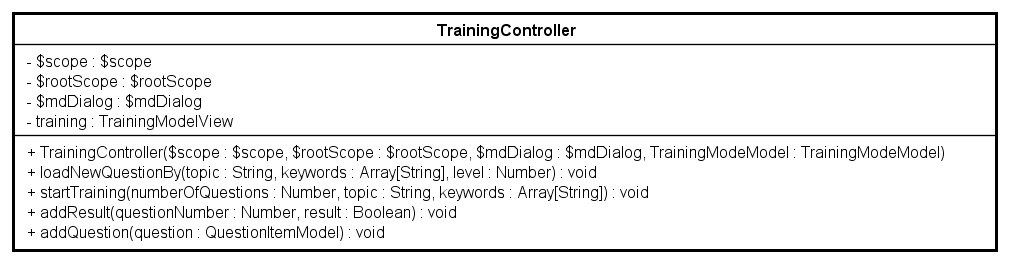
\includegraphics[scale=0.45]{UML/Classi/Front-End/QuizziPedia_Front-end_Controller_TrainingController.png}
	\caption{QuizziPedia::Front-End::Controllers::TrainingController}
\end{figure} \FloatBarrier
\begin{itemize}
	\item \textbf{Descrizione}: questa classe permette di gestire la modalità allenamento sottoponendo all'utente le giuste domande adatte al suo livello;
	\item \textbf{Utilizzo}: fornisce le funzionalità per recuperare le domande che siano in accordo con il livello dell'utente;
	\item \textbf{Relazione con altre classi}:
	\begin{itemize}
		\item \textit{IN} \texttt{TrainingModelView}: ;
		\item \textit{IN} \texttt{TrainingModeModel}: ;
		\item \textit{IN} \texttt{TrainingSetUpTemplate}: rappresenta il componente grafico che permette all'utente di selezionare l'argomento e le parole chiave per iniziare un allenamento con queste caratteristiche. Viene gestito dinamicamente all'interno della view TrainingView attraverso il controller TrainingController;
		\item \textit{IN} \texttt{QuestionController}: ;
		\item \textit{IN} \texttt{QuestionItemMode}: ;
	\end{itemize}
	\item \textbf{Attributi}:
	\begin{itemize}
		\item \texttt{-} \texttt{\$scope: \$scope} \\
		Campo dati contenente un riferimento all’oggetto \$scope creato da \textit{Angular\ped{G}}, viene utilizzato come mezzo di comunicazione tra il controller e la view. Contiene gli oggetti che definiscono il model dell’applicazione;
		\item \texttt{-} \texttt{\$rootScope: \$rootScope} \\
		Campo dati contenente il riferimento all'oggetto globale \$rootScope creato da \textit{Angular\ped{G}}. Viene utilizzato per rendere accessibile a tutti i controller e a tutte le view l'oggetto \texttt{TrainingModeModel}. In questo caso viene utilizzato per inserire in \$rootScope l'oggetto di ritorno della chiamata a \texttt{getNextQuestion};
		\item \texttt{-} \texttt{\$mdDialog: \$mdDialog} \\
		Campo dati contenente un riferimento al servizio della libreria \textit{Material for Angular\ped{G}} che permette di creare delle componenti a popup;
		\item \texttt{+} \texttt{training: TrainingModelView} \\
		Oggetto di tipo \texttt{TrainingModelView}. All'interno di esso sono presenti le variabili e i metodi necessari per il \textit{Two-Way Data-Binding\ped{G}} tra la view \texttt{TrainingView} e il controller \texttt{TrainingController};
	\end{itemize}
	\item \textbf{Metodi}:
	\begin{itemize}
		\item \texttt{+} \texttt{TrainingController(\$scope: \$scope, \$rootscope: \$rootscope, \$mdDialog: \$mdDialog)} \\ Metodo costruttore della classe; \\
		\textbf{Parametri:}
		\begin{itemize}
			\item \texttt{\$scope: \$scope} \\
			Parametro contenente un riferimento all’oggetto \$scope creato da \textit{Angular\ped{G}}. Viene utilizzato come mezzo di comunicazione tra il controller e la view. Contiene gli oggetti che definiscono il viewmodel e il model dell’applicazione;
			\item \texttt{\$rootscope: \$rootscope}\\
			Parametro contenente il riferimento all'oggetto globale \$rootScope creato da \textit{Angular\ped{G}}. Viene utilizzato per rendere accessibile a tutti i controller e a tutte le view l'oggetto \texttt{UserDetailsModel}. In questo caso viene utilizzato per aggiornare in \$rootScope l'oggetto che rappresenta l'utente autenticato all'interno dell'applicazione;
			\item \texttt{\$mdDialog: \$mdDialog} \\
			Parametro contenente un riferimento al servizio della libreria \textit{Material for Angular\ped{G}} che permette di creare delle componenti a popup.
		\end{itemize}
		\item \texttt{-} \texttt{getNextQuestion(): QuestionItemModel} \\ Metodo che gestisce l'evento del click al pulsante "prossima domanda", fa una richiesta al QuestionController che ritornerà la domanda successiva. Questa domanda andrà salvata nel TrainingModeModel nello \$scope.
	\end{itemize}
\end{itemize}

\paragraph{QuizziPedia::Front-End::Controllers::FillingQuestionnaireController}
\begin{figure} [ht]
	\centering
	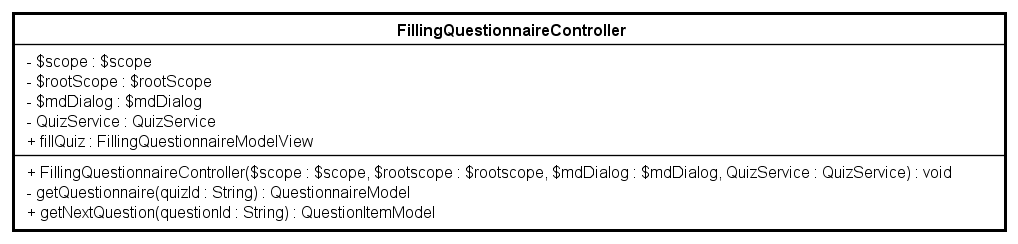
\includegraphics[scale=0.45]{UML/Classi/Front-End/QuizziPedia_Front-end_Controller_FillingQuestionnaireController.png}
	\caption{QuizziPedia::Front-End::Controllers::FillingQuestionnaireController}
\end{figure} \FloatBarrier
\begin{itemize}
	\item \textbf{Descrizione}: questa classe permette di gestire la compilazione del questionario;
	\item \textbf{Utilizzo}: fornisce le funzionalità per compilare un questionario e per gestire il cambio di domanda;
	\item \textbf{Relazione con altre classi}:
	\begin{itemize}
		\item \textit{IN} \texttt{FillingQuestionnaireModelView}: ;  
		\item \textit{IN} \texttt{InfoQuestionnaireTemplate}: rappresenta il componente grafico che permette all'utente di visualizzare le informazioni principali del questionario che si sta per svolgere. Viene gestito dinamicamente all'interno della view TrainingView attraverso il controller TrainingController;
		\item \textit{IN} \texttt{QuizService}: permette di ottenere i dati di un quiz tramite delle parole chiave inserite dall'utente nella barra di ricerca. Permette inoltre di iscriversi ad un questionario e di scaricare l'intera l'ista di domande di un questionario a partire dal suo id univoco;
		\item \textit{IN} \texttt{QuestionnaireModel}: ;
		\item \textit{IN} \texttt{QuestionsController}: ; 
		\item \textit{IN} \texttt{QuestionItemModel}: ;
	\end{itemize}
	\item \textbf{Attributi}:
	\begin{itemize}
		\item \texttt{-} \texttt{\$scope: \$scope} \\
		Campo dati contenente un riferimento all’oggetto \$scope creato da \textit{Angular\ped{G}}, viene utilizzato come mezzo di comunicazione tra il controller e la view. Contiene gli oggetti che definiscono il model dell’applicazione;
		\item \texttt{-} \texttt{\$rootScope: \$rootScope} \\
		Campo dati contenente il riferimento all'oggetto globale \$rootScope creato da \textit{Angular\ped{G}}. Viene utilizzato per rendere accessibile a tutti i controller e a tutte le view l'oggetto \texttt{QuestionnaireModel}. In questo caso viene utilizzato per inserire in \$rootScope l'oggetto di ritorno della chiamata a \texttt{getNextQuestion} e l'intero questionario ritornato dalla chiamata a \texttt{getQuestionnaire};
		\item \texttt{-} \texttt{\$mdDialog: \$mdDialog} \\
		Campo dati contenente un riferimento al servizio della libreria \textit{Material for Angular\ped{G}} che permette di creare delle componenti a popup;
		\item \texttt{-} \texttt{QuizService: QuizService}: ;
		\item \texttt{+} \texttt{fillQuiz: FillingQuestionnaireModelView} \\
		Oggetto di tipo \texttt{FillingQuestionnaireModelView}. All'interno di esso sono presenti le variabili e i metodi necessari per il \textit{Two-Way Data-Binding\ped{G}} tra la view \texttt{FillingQuestionnaireView} e il controller \texttt{FillingQuestionnaireController};
	\end{itemize}
	\item \textbf{Metodi}:
	\begin{itemize}
		\item \texttt{+} \texttt{FillingQuestionnaireController(\$scope: \$scope, \$rootscope: \$rootscope, \$mdDialog: \$mdDialog, QuizService: QuizService)} \\Metodo costruttore della classe.\\
		\textbf{Parametri}:
		\begin{itemize}
			\item \texttt{-} \texttt{\$scope: \$scope} \\
			Campo dati contenente un riferimento all’oggetto \$scope creato da \textit{Angular\ped{G}}. Viene utilizzato come mezzo di comunicazione tra il controller e la view. Contiene gli oggetti che definiscono il viewmodel e il model dell’applicazione;
			\item \texttt{-} \texttt{\$location: \$location} \\
			Campo dati contenente un riferimento al servizio creato da \textit{Angular\ped{G}} che permette di accedere alla barra degli indirizzi del \textit{browser\ped{G}}, i cambiamenti all’URL nella barra degli indirizzi si riflettono in questo oggetto e viceversa;
			\item \texttt{-} \texttt{\$mdDialog: \$mdDialog} \\
			Campo dati contenente un riferimento al servizio della libreria \textit{Material for Angular\ped{G}} che permette di creare delle componenti a popup;
			\item \texttt{QuizService: QuizService}: parametro che permette di ottenere, tramite il service, la lista di tutte le domande presenti nel quiz;
		\end{itemize}
		\item \texttt{+} \texttt{getQuestionnaire(quizId: String): QuestionnaireModel}: \\ Metodo che permette di ottenere l'intero questionario; \\
		\textbf{Parametri}:
		\begin{itemize}
			\item \texttt{quizId: String}: parametro che indica l'id del quiz che vogliamo ricevere dal back-end.
		\end{itemize}
		\item \texttt{+} \texttt{getNextQuestion(questionId: String): QuestionItemModel}: \\ Metodo che ritorna la domanda successiva del quiz tramite chiamata a QuestionController; \\
		\textbf{Parametri}:
		\begin{itemize}
			\item \texttt{questionId: String}: parametro che indica l'id della domanda che vogliamo ricevere dal back-end.
		\end{itemize}
	\end{itemize}
\end{itemize}

\paragraph{QuizziPedia::Front-End::Controllers::CreateQuestionnaireController}
\begin{figure} [ht]
	\centering
	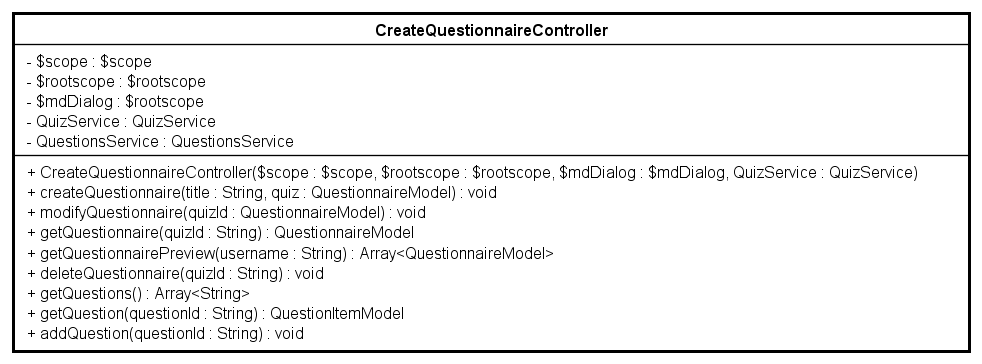
\includegraphics[scale=0.45]{UML/Classi/Front-End/QuizziPedia_Front-end_Controller_CreateQuestionnaireController.png}
	\caption{QuizziPedia::Front-End::Controllers::CreateQuestionnaireController}
\end{figure} \FloatBarrier
\begin{itemize}
	\item \textbf{Descrizione}: questa classe permette di gestire la creazione di un questionario;
	\item \textbf{Utilizzo}: fornisce tutte le funzionalità per la creazione di un nuovo questionario e per la modifica di uno esistente;
	\item \textbf{Relazione con altre classi}:
	\begin{itemize}
		\item \textit{IN} \texttt{CreateQuestionnaireModelView}: view per la creazione del questionario; 
		\item \textit{IN} \texttt{QuizService}: questa classe permette di ottenere i dati di un quiz tramite delle parole chiave inserite dall'utente nella barra di ricerca;
		\item \textit{IN} \texttt{QuestionnaireModel}: ;
	\end{itemize}
	\item \textbf{Attributi}:
	\begin{itemize}
		\item \texttt{-} \texttt{\$scope: \$scope} \\
		Campo dati contenente un riferimento all’oggetto \$scope creato da \textit{Angular\ped{G}}, viene utilizzato come mezzo di comunicazione tra il controller e la view. Contiene gli oggetti che definiscono il model dell’applicazione;
		\item \texttt{-} \texttt{\$rootScope: \$rootScope} \\
		Campo dati contenente il riferimento all'oggetto globale \$rootScope creato da \textit{Angular\ped{G}}. Viene utilizzato per rendere accessibile a tutti i controller e a tutte le view l'oggetto \texttt{QuestionnaireModel}. In questo caso viene utilizzato per inserire in \$rootScope l'oggetto di ritorno della chiamata a \texttt{getQuestiontionnaire} e la lista dei questionari ottenuta dalla chiamata \texttt{getQuestionnairePreview};
		\item \texttt{-} \texttt{\$mdDialog: \$mdDialog} \\
		Campo dati contenente un riferimento al servizio della libreria \textit{Material for Angular\ped{G}} che permette di creare delle componenti a popup;
		\item \texttt{-} \texttt{QuizService}: ;
	\end{itemize}
	\item \textbf{Metodi}:
	\begin{itemize}
		\item \texttt{+} \texttt{CreateQuestionnaireController(\$scope: \$scope, \$rootscope: \$rootscope, \$mdDialog: \$mdDialog, QuizService: QuizService)}: \\ Metodo costruttore della classe. \\
		\textbf{Parametri}:
		\begin{itemize}
			\item \texttt{-} \texttt{\$scope: \$scope} \\
			Campo dati contenente un riferimento all’oggetto \$scope creato da \textit{Angular\ped{G}}. Viene utilizzato come mezzo di comunicazione tra il controller e la view. Contiene gli oggetti che definiscono il viewmodel e il model dell’applicazione;
				\item \texttt{-} \texttt{\$rootScope: \$rootScope} \\
				Campo dati contenente il riferimento all'oggetto globale \$rootScope creato da \textit{Angular\ped{G}}. Viene utilizzato per rendere accessibile a tutti i controller e a tutte le view l'oggetto \texttt{QuestionnaireModel}. In questo caso viene utilizzato per inserire in \$rootScope l'oggetto di ritorno della chiamata a \texttt{getQuestiontionnaire} e la lista dei questionari ottenuta dalla chiamata \texttt{getQuestionnairePreview};
			\item \texttt{-} \texttt{\$mdDialog: \$mdDialog} \\
			Campo dati contenente un riferimento al servizio della libreria \textit{Material for Angular\ped{G}} che permette di creare delle componenti a popup;
			\item \texttt{QuizService: QuizService}: parametro che permette di ottenere, tramite il service, la lista di tutte le domande presenti nel quiz;
		\end{itemize}
		\item \texttt{+} \texttt{createQuestionnaire(title: String, quiz: QuestionnaireModel)}: \\Metodo che permette di inserire un questionario nel database tramite richiesta al service; \\
			\textbf{Parametri}:
			\begin{itemize}
				\item 
			\end{itemize}
		\item \texttt{+} \texttt{modifyQuestionnaire(quizId: QuestionnaireModel)}: \\ Metodo che serve per modificare un questionario; \\
			\textbf{Parametri}:
			\begin{itemize}
				\item \texttt{quiz: QuestionnaireModel}: parametro che rappresenta l'oggetto questionario;
			\end{itemize}
		\item \texttt{+} \texttt{getQuestionnaire(quizId: String)}: \\Metodo che serve per ottenere un questionario tramite l'id in modo da poterlo modificare; \\
			\textbf{Parametri}:
			\begin{itemize}
				\item \texttt{quizId: String}: parametro che rappresenta l'id del questionario da richiedere.
			\end{itemize}
		\item \texttt{+} \texttt{getQuestionnairePreview(username: String)}: \\ Metodo che serve per ottenere la lista di tutti i questionari di un utente; \\
			\textbf{Parametri}:
			\begin{itemize}
				\item \texttt{username: String}: parametro che indica l'utente del quale vogliamo caricare tutti i questionari.
			\end{itemize}
		\item \texttt{+} \texttt{deleteQuestionnaire(quizId: String): void}: \\Metodo che elimina un questionario.
		\textbf{Parametri}:
		\texttt{quizId: String}: identificativo del questionario da eliminare.
	\end{itemize}
\end{itemize}

\paragraph{QuizziPedia::Front-End::Controllers::RegistrationManagementController}
\begin{figure} [ht]
	\centering
	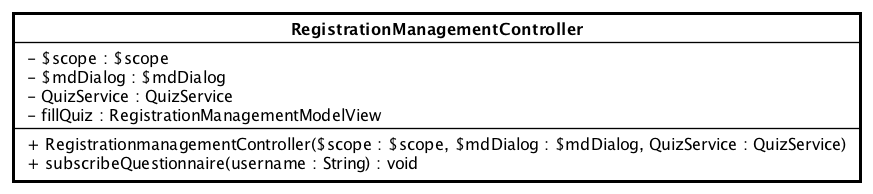
\includegraphics[scale=0.45]{UML/Classi/Front-End/QuizziPedia_Front-end_Controller_RegistrationManagementController.png}
	\caption{QuizziPedia::Front-End::Controllers::RegistrationManagementController}
\end{figure} \FloatBarrier
\begin{itemize}
	\item \textbf{Descrizione}: questa classe permette di gestire le iscrizione degli utenti ai questionari;
	\item \textbf{Utilizzo}: fornisce le funzionalità di iscrizione ad un questionario;
	\item \textbf{Relazione con altre classi}:
	\begin{itemize}
		\item \textit{IN} \texttt{RegistratioManagementModelView}: ; 
		\item \textit{OUT} \texttt{QuizService}: questa classe permette di ottenere i dati di un quiz tramite delle parole chiave inserite dall'utente nella barra di ricerca;
	\end{itemize}
	\item \textbf{Attributi}:
	\begin{itemize}
		\item \texttt{-} \texttt{\$scope: \$scope} \\
		Campo dati contenente un riferimento all’oggetto \$scope creato da \textit{Angular\ped{G}}, viene utilizzato come mezzo di comunicazione tra il controller e la view. Contiene gli oggetti che definiscono il model dell’applicazione;
		\item \texttt{-} \texttt{\$mdDialog: \$mdDialog} \\
		Campo dati contenente un riferimento al servizio della libreria \textit{Material for Angular\ped{G}} che permette di creare delle componenti a popup;
		\item \texttt{QuizService: QuizService}: parametro che permette di ottenere, tramite il service, la lista di tutte le domande presenti nel quiz;
	\end{itemize}
	\item \textbf{Metodi}:
	\begin{itemize}
		\item \texttt{RegistrationmanagementController(\$scope: \$scope, \$mdDialog: \$mdDialog, QuizService: QuizService)}: \\Metodo costruttore della classe. \\
			\textbf{Parametri}:
			\begin{itemize}
					\item \texttt{-} \texttt{\$scope: \$scope} \\
					Campo dati contenente un riferimento all’oggetto \$scope creato da \textit{Angular\ped{G}}. Viene utilizzato come mezzo di comunicazione tra il controller e la view. Contiene gli oggetti che definiscono il viewmodel e il model dell’applicazione;
					\item \texttt{-} \texttt{\$mdDialog: \$mdDialog} \\
					Campo dati contenente un riferimento al servizio della libreria \textit{Material for Angular\ped{G}} che permette di creare delle componenti a popup;
					\item \texttt{-} \texttt{QuizService: QuizService}: parametro che permette di ottenere, tramite il service, la lista di tutte le domande presenti nel quiz; 
			\end{itemize}
		\item \texttt{subscribeQuestionnaire(username: String): void} \\ Metodo che permette l'iscrizione ad un questionario. Richiama la funzionalità del QuizService. \\
		\textbf{Parametri}:
		\begin{itemize}
			\item \texttt{username: String}: parametro che indica l'utente da iscrivere al questionario.
		\end{itemize}
	\end{itemize}
\end{itemize}

\paragraph{QuizziPedia::Front-End::Controllers::ResultsController}
\begin{figure} [ht]
	\centering
	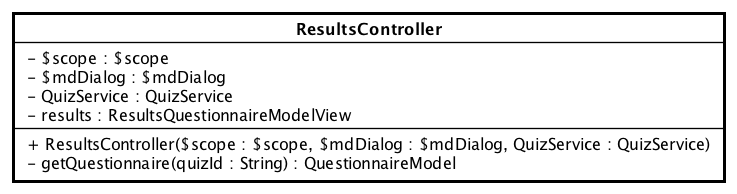
\includegraphics[scale=0.45]{UML/Classi/Front-End/QuizziPedia_Front-end_Controller_ResultsController.png}
	\caption{QuizziPedia::Front-End::Controllers::ResultsController}
\end{figure} \FloatBarrier
\begin{itemize}
	\item \textbf{Descrizione}: questa classe permette di gestire i risultati della ricerca effettuata dall'utente;
	\item \textbf{Utilizzo}: fornisce le funzionalità per recuperare i dati dal back-end e mostrarli all'utente nella view;
	\item \textbf{Relazione con altre classi}:
	\begin{itemize}
		\item \textit{IN} \texttt{ResultsQuestionnaireModelView}: ; 
		\item \textit{IN} \texttt{QuizService}: questa classe permette di ottenere i dati di un quiz tramite delle parole chiave inserite dall'utente nella barra di ricerca;
		\item \textit{IN} \texttt{QuestionnaireModel}: ;
	\end{itemize}
	\item \textbf{Attributi}:
	\begin{itemize}
		\item \texttt{-} \texttt{\$scope: \$scope} \\
		Campo dati contenente un riferimento all’oggetto \$scope creato da \textit{Angular\ped{G}}, viene utilizzato come mezzo di comunicazione tra il controller e la view. Contiene gli oggetti che definiscono il model dell’applicazione;
		\item \texttt{-} \texttt{\$mdDialog: \$mdDialog} \\
		Campo dati contenente un riferimento al servizio della libreria \textit{Material for Angular\ped{G}} che permette di creare delle componenti a popup;
		\item \textit{-} \texttt{QuizService}: questa classe permette di ottenere i dati di un quiz tramite delle parole chiave inserite dall'utente nella barra di ricerca;
	\end{itemize}
	\item \textbf{Metodi}:
	\begin{itemize}
		\item \texttt{+} \texttt{ResultsController(\$scope: \$scope, \$mdDialog: \$mdDialog), QuizService: QuizService}: \\Metodo costruttore della classe. \\
		\textbf{Parametri}: 
		\begin{itemize}
			\item \texttt{-} \texttt{\$scope: \$scope} \\
			Campo dati contenente un riferimento all’oggetto \$scope creato da \textit{Angular\ped{G}}. Viene utilizzato come mezzo di comunicazione tra il controller e la view. Contiene gli oggetti che definiscono il viewmodel e il model dell’applicazione;
			\item \texttt{-} \texttt{\$mdDialog: \$mdDialog} \\
			Campo dati contenente un riferimento al servizio della libreria \textit{Material for Angular\ped{G}} che permette di creare delle componenti a popup;
			\item \texttt{-} \texttt{QuizService: QuizService}: parametro che permette di ottenere, tramite il service, la lista di tutte le domande presenti nel quiz;
		\end{itemize}
		\item \texttt{-} \texttt{getQuestionnaire(quizId: String): QuestionnaireModel}: \\Metodo che ritorna tutti i dati di un questionario.\\
		\textbf{Parametri}:
		\begin{itemize}
			\item \texttt{quizId: String}: parametro che indica l'id univoco del questionario da caricare.
		\end{itemize}
	\end{itemize}
\end{itemize}

\paragraph{QuizziPedia::Front-End::Controllers::QuestionnaireManagementController}
\begin{figure} [ht]
	\centering
	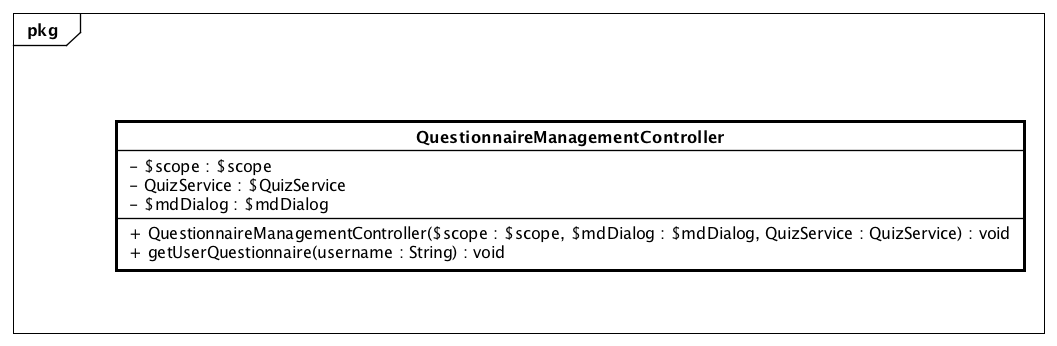
\includegraphics[scale=0.45]{UML/Classi/Front-End/QuizziPedia_Front-end_Controller_QuestionnaireManagementController.png}
	\caption{QuizziPedia::Front-End::Controllers::QuestionnaireManagementController}
\end{figure} \FloatBarrier
\begin{itemize}
	\item \textbf{Descrizione}: questa classe permette di gestire tutti i questionari creati da un utente; 
	\item \textbf{Utilizzo}: fornisce le funzionalità per recuperare dal back-end tutti i questionari creati da un utente;
	\item \textbf{Relazione con altre classi}:
	\begin{itemize}
		\item \textit{IN} \texttt{QuestionnaireManagementeModelView}: ;
		\item \textit{IN} \texttt{QuizService}: questa classe permette di ottenere i dati di un quiz tramite delle parole chiave inserite dall'utente nella barra di ricerca;
		\item \texttt{-} \texttt{\$mdDialog: \$mdDialog} \\
		Campo dati contenente un riferimento al servizio della libreria \textit{Material for Angular\ped{G}} che permette di creare delle componenti a popup;
		\item \textit{IN} \texttt{QuestionnaireModel}: ;
	\end{itemize}
	\item \textbf{Attributi}:
	\begin{itemize}
		\item \texttt{-} \texttt{\$scope: \$scope} \\
		Campo dati contenente un riferimento all’oggetto \$scope creato da \textit{Angular\ped{G}}, viene utilizzato come mezzo di comunicazione tra il controller e la view. Contiene gli oggetti che definiscono il model dell’applicazione;
		\item \textit{IN} \texttt{QuizService}: permette di ottenere i dati di un quiz tramite delle parole chiave inserite dall'utente nella barra di ricerca;
	\end{itemize}
	\item \textbf{Metodi}:
	\begin{itemize}
		\item \texttt{+} \texttt{QuestionnaireManagementController(\$scope: \$scope, \$mdDialog: \$mdDialog, QuizService: QuizService)}: \\Metodo costruttore della classe;\\
		\textbf{Parametri}: 
		\begin{itemize}
			\item \texttt{-} \texttt{\$scope: \$scope} \\
			Campo dati contenente un riferimento all’oggetto \$scope creato da \textit{Angular\ped{G}}. Viene utilizzato come mezzo di comunicazione tra il controller e la view. Contiene gli oggetti che definiscono il viewmodel e il model dell’applicazione;
			\item \texttt{-} \texttt{\$mdDialog: \$mdDialog} \\
			Campo dati contenente un riferimento al servizio della libreria \textit{Material for Angular\ped{G}} che permette di creare delle componenti a popup;
			\item \texttt{-} \texttt{QuizService: QuizService}: parametro che permette di ottenere, tramite il service, la lista di tutte le domande presenti nel quiz;
		\end{itemize}
		\item \texttt{-} \texttt{getUserQuestionnaire(username: String) QuestionnaireModel[]}: \\Metodo che ritorna tutti i questionari creati da un utente in un array di QuestionnaireModel.
		\textbf{Parametri}:
		\begin{itemize}
			\item \texttt{username: String}: parametro che indica l'identificativo dell'utente del quale vogliamo scaricare tutti i questionari.
		\end{itemize}
	\end{itemize}
\end{itemize}

\paragraph{QuizziPedia::Front-End::Controllers::QuestionnaireDetailsController}
\begin{figure} [ht]
	\centering
	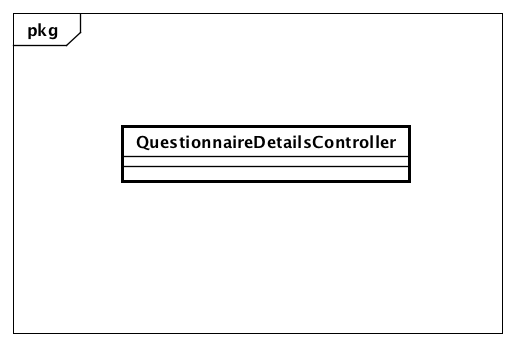
\includegraphics[scale=0.45]{UML/Classi/Front-End/QuizziPedia_Front-end_Controller_QuestionnaireDetailsController.png}
	\caption{QuizziPedia::Front-End::Controllers::QuestionnaireDetailsController}
\end{figure} \FloatBarrier
\begin{itemize}
	\item \textbf{Descrizione}: questa classe permette di gestire i dettagli di un questionario; 
	\item \textbf{Utilizzo}: fornisce le funzionalità per recuperare dal back-end i dettagli di un questionario creato da un utente al fine di poterli visualizzare nel suo profilo;
	\item \textbf{Relazione con altre classi}:
	\begin{itemize}
		\item \textit{IN} \texttt{QuestionnaireDetailsModelView}: ;
		\item \textit{IN} \texttt{QuizService}: questa classe permette di ottenere i dati di un quiz tramite delle parole chiave inserite dall'utente nella barra di ricerca;
		\item \textit{} \texttt{QuestionnaireModel}: ;
	\end{itemize}
	\item \textbf{Attributi}:
	\begin{itemize}
		\item \texttt{-} \texttt{\$scope: \$scope} \\
		Campo dati contenente un riferimento all’oggetto \$scope creato da \textit{Angular\ped{G}}, viene utilizzato come mezzo di comunicazione tra il controller e la view. Contiene gli oggetti che definiscono il model dell’applicazione;
		\item \texttt{-} \texttt{\$rootScope: \$rootScope} \\
		Campo dati contenente il riferimento all'oggetto globale \$rootScope creato da \textit{Angular\ped{G}}. Viene utilizzato per rendere accessibile a tutti i controller e a tutte le view l'oggetto \texttt{QuestionnaireModel}. In questo caso viene utilizzato per inserire in \$rootScope l'oggetto di ritorno della chiamata a \texttt{getQuestionnaireDetails} del service \texttt{QuizService};
		\item \texttt{-} \texttt{QuizService}: permette di ottenere i dati di un quiz tramite delle parole chiave inserite dall'utente nella barra di ricerca;
	\end{itemize}
	\item \textbf{Metodi}:
	\begin{itemize}
		\item \texttt{+} \texttt{QuestionnaireDetailsController(\$scope: \$scope, \$rootscope: \$rootscope, \$mdDialog: \$mdDialog, QuizService: QuizService)}: \\ Metodo costruttore della classe;
		\textbf{Parametri}: 
		\begin{itemize}
			\item \texttt{-} \texttt{\$scope: \$scope} \\
			Campo dati contenente un riferimento all’oggetto \$scope creato da \textit{Angular\ped{G}}. Viene utilizzato come mezzo di comunicazione tra il controller e la view. Contiene gli oggetti che definiscono il viewmodel e il model dell’applicazione;
			\item \texttt{-} \texttt{\$rootScope: \$rootScope} \\
			Campo dati contenente il riferimento all'oggetto globale \$rootScope creato da \textit{Angular\ped{G}}. Viene utilizzato per rendere accessibile a tutti i controller e a tutte le view l'oggetto \texttt{QuestionnaireModel}. In questo caso viene utilizzato per inserire in \$rootScope l'oggetto di ritorno della chiamata a \texttt{getQuestionnaireDetails} del service \texttt{QuizService};	
			\item \texttt{-} \texttt{\$mdDialog: \$mdDialog} \\
			Campo dati contenente un riferimento al servizio della libreria \textit{Material for Angular\ped{G}} che permette di creare delle componenti a popup;
			\item \texttt{-} \texttt{QuizService: QuizService}: parametro che permette di ottenere, tramite il service, la lista di tutte le domande presenti nel quiz;
		\end{itemize}
		
		\item \texttt{-} \texttt{getQuestionnaireDetails(username: String)}: \\ Metodo che richiede al service i dettagli dei questionari eseguiti dall'utente.
		\textbf{Parametri}:
		\begin{itemize}
			\item \texttt{username: String}: username dell'utente del quale caricare i questionari.
		\end{itemize}
		\item \texttt{-} \texttt{getSubscribedQuestionnaire(username: String)}: \\Metodo che ritorna i questionari a cui l'utente è iscritto.
		\textbf{Parametri}:
		\begin{itemize}
			\item \texttt{username: String}: identificativo dell'utente del quale scaricare i questionari a cui è iscritto.
		\end{itemize}
	\end{itemize}
\end{itemize}

\paragraph{QuizziPedia::Front-End::Controllers::UserDetailsController}
\begin{figure} [ht]
	\centering
	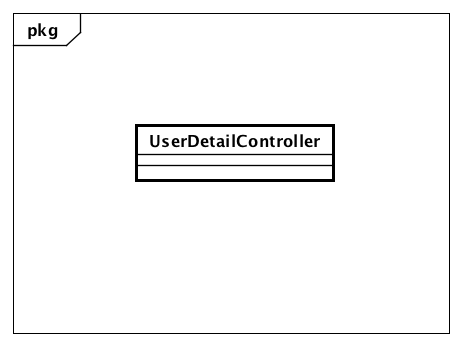
\includegraphics[scale=0.45]{UML/Classi/Front-End/QuizziPedia_Front-end_Controller_UserDetailController.png}
	\caption{QuizziPedia::Front-End::Controllers::UserDetailController}
\end{figure} \FloatBarrier
\begin{itemize}
	\item \textbf{Descrizione}: questa classe permette di ottenere i dati di un utente;
	\item \textbf{Utilizzo}: fornisce le funzionalità per ottenere i dati di un utente per poterle mostrare nella view;
	\item \textbf{Relazione con altre classi}:
	\begin{itemize}
		\item \textit{IN} \texttt{UserDetailsModelView}: directive che permette di visualizzare i dati di un utente; 
		\item \textit{IN} \texttt{UserDetailsService}: questa classe permette di ottenere i dati dell'utente;
		\item \textit{IN} \texttt{UserDetailsModel}: 
	\end{itemize}
	\item \textbf{Attributi}:
	\begin{itemize}
		\item \texttt{-} \texttt{\$scope: \$scope} \\
		Campo dati contenente un riferimento all’oggetto \$scope creato da \textit{Angular\ped{G}}, viene utilizzato come mezzo di comunicazione tra il controller e la view. Contiene gli oggetti che definiscono il model dell’applicazione;
		\item \texttt{-} \texttt{\$rootScope: \$rootScope} \\
		Campo dati contenente il riferimento all'oggetto globale \$rootScope creato da \textit{Angular\ped{G}}. Viene utilizzato per rendere accessibile a tutti i controller e a tutte le view l'oggetto \texttt{UserDetailsModel}. In questo caso viene utilizzato per inserire in \$rootScope l'oggetto di ritorno della chiamata a \texttt{getUserDetails} del service \texttt{UserDetailsService};
		\item \texttt{-} \texttt{userDetailsService}: parametro permette di ottenere i dati dell'utente;
		\item \texttt{-} \texttt{UserDetailsService}: parametro che permette di ottenere i dati dell'utente;
	\end{itemize}	
	\begin{itemize}
		\item \textbf{Metodi}:
		\item \texttt{+} \texttt{UserDetailsController(\$scope: \$scope, \$rootscope:\$rootscope, \$mdDialog: \$mdDialog, UserDetailsService: UserDetailsService)} \\ Metodo costruttore della classe;\\
		\textbf{Parametri}: 
		\begin{itemize}
			\item \texttt{-} \texttt{\$scope: \$scope} \\
			Campo dati contenente un riferimento all’oggetto \$scope creato da \textit{Angular\ped{G}}. Viene utilizzato come mezzo di comunicazione tra il controller e la view. Contiene gli oggetti che definiscono il viewmodel e il model dell’applicazione;
			\item \texttt{-} \texttt{\$rootScope: \$rootScope} \\
			Parametro contenente il riferimento all'oggetto globale \$rootScope creato da \textit{Angular\ped{G}}. Viene utilizzato per rendere accessibile a tutti i controller e a tutte le view l'oggetto \texttt{UserDetailsModel}. In questo caso viene utilizzato per inserire in \$rootScope l'oggetto di ritorno della chiamata a \texttt{getUserDetails} del service \texttt{UserDetailsService};
			\item \texttt{-} \texttt{\$mdDialog: \$mdDialog} \\
			Campo dati contenente un riferimento al servizio della libreria \textit{Material for Angular\ped{G}} che permette di creare delle componenti a popup;
			\item \texttt{-} \texttt{userDetailsService: userDetailsService}: parametro che permette di ottenere, tramite il service, la lista di tutti i dati dell'utente;
		\end{itemize}
		\item \texttt{-} \texttt{getUserDetails(username: String): UserDetailsModel} \\ Metodo che permette di ottenere i dati con una chiamata a UserDetailsService;
		\textbf{Parametri}:
		\begin{itemize}
			\item \texttt{username: String}: parametro che identifica l'utente del quale saranno scaricati i dati.
		\end{itemize}
	\end{itemize}
\end{itemize}

\paragraph{QuizziPedia::Front-End::Controllers::QuestionsController}
\begin{figure} [ht]
	\centering
	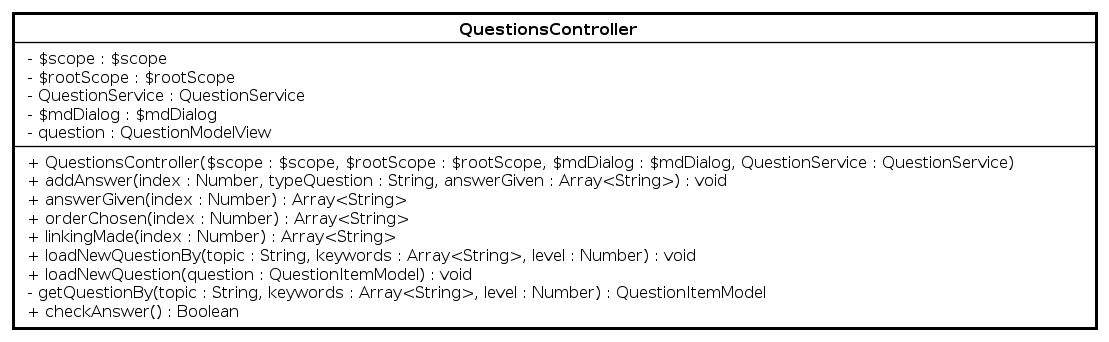
\includegraphics[scale=0.45]{UML/Classi/Front-End/QuizziPedia_Front-end_Controller_QuestionsController.png}
	\caption{QuizziPedia::Front-End::Controllers::QuestionsController}
\end{figure} \FloatBarrier
\begin{itemize}
	\item \textbf{Descrizione}: questa classe permette di gestire il recupero delle domande per poterle stampare nella modalità allenamento;
	\item \textbf{Utilizzo}: fornisce le funzionalità per il recupero delle domande esistenti nel database al fine di mostrarle durante la modalità allenamento nell'apposito template;
	\item \textbf{Relazione con altre classi}:
	\begin{itemize}
		\item \textit{IN} \texttt{HeaderTextQuestionTemplate}: rappresenta il componente grafico che presenta all'utente il testo della domanda, l'argomento e le parole chiave. Viene gestito dinamicamente all'interno della view TrainingView attraverso il controller TrainingController; 
		\item \textit{IN} \texttt{TrueFalseAnswerTemplate}: rappresenta il componente grafico che permette all'utente di visualizzare la domanda vero e falso. Viene gestito dinamicamente all'interno della view TrainingView attraverso il controller TrainingController; 
		\item \textit{IN} \texttt{MultipleChoiceAnswerTemplate}: rappresenta il componente grafico che permette all'utente di visualizzare la domanda a risposta multipla. Viene gestito dinamicamente all'interno della view TrainingView attraverso il controller TrainingController; 
		\item \textit{IN} \texttt{LinkingAnswerTemplate}: rappresenta il componente grafico che permette all'utente di visualizzare la domanda di collegamento. Viene gestito dinamicamente all'interno della view TrainingView attraverso il controller TrainingController; 
		\item \textit{IN} \texttt{SortImagesAnswerTemplate}: rappresenta il componente grafico che permette all'utente di visualizzare la domanda ad ordinamento di immagini. Viene gestito dinamicamente all'interno della view TrainingView attraverso il controller TrainingController; 
		\item \textit{IN} \texttt{SortTextAnswerTemplate}: rappresenta il componente grafico che permette all'utente di visualizzare la domanda ad ordinamento di stringhe. Viene gestito dinamicamente all'interno della view TrainingView attraverso il controller TrainingController; 
		\item \textit{IN} \texttt{EmptySpaceAnswerTemplate}: rappresenta il componente grafico che permette all'utente di visualizzare l'esercizio a riempimento di spazi vuoti. Viene gestito dinamicamente all'interno della view TrainingView attraverso il controller TrainingController; 
		\item \textit{IN} \texttt{ClickableAnswerTemplate}: rappresenta il componente grafico che permette all'utente di visualizzare la domanda ad area cliccabile nell'immagine. Viene gestito dinamicamente all'interno della view TrainingView attraverso il controller TrainingController;  
		\item \textit{IN} \texttt{QuestionServices}: questa classe permette di ottenere domande esistenti e salvare nuove domande;
		\item \textit{IN} \texttt{QuestionItemModel}: ;
		\item \textit{OUT} \texttt{FillingQuestionnaireController}: ;
		
	\end{itemize}
	\item \textbf{Attributi}:
	\begin{itemize}
		\item \texttt{-} \texttt{\$scope: \$scope} \\
		Campo dati contenente un riferimento all’oggetto \$scope creato da \textit{Angular\ped{G}}, viene utilizzato come mezzo di comunicazione tra il controller e la view. Contiene gli oggetti che definiscono il model dell’applicazione;
		\item \texttt{-} \texttt{\$rootScope: \$rootScope} \\
		Campo dati contenente il riferimento all'oggetto globale \$rootScope creato da \textit{Angular\ped{G}}. Viene utilizzato per rendere accessibile a tutti i controller e a tutte le view l'oggetto \texttt{QuestionItemModel}. In questo caso viene utilizzato per inserire in \$rootScope l'oggetto di ritorno della chiamata a \texttt{getQuestion} del service \texttt{QuestionService};
		\item \texttt{-} \texttt{QuestionService}: ;
	\end{itemize}
	\item \textbf{Metodi}:
	\begin{itemize}
		\item \texttt{+} \texttt{QuestionsController}: \\ Metodo costruttore della classe
		\item \texttt{+} \texttt{getQuestion}: \\ Metodo che richiede al back-end una domanda;
	\end{itemize}
\end{itemize}

\paragraph{QuizziPedia::Front-End::Controllers::TopicKeywordsController}
\begin{figure} [ht]
	\centering
	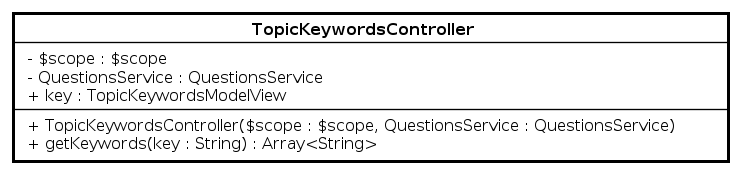
\includegraphics[scale=0.45]{UML/Classi/Front-End/QuizziPedia_Front-end_Controller_TopicKeywordsController.png}
	\caption{QuizziPedia::Front-End::Controllers::TopicKeywordsController}
\end{figure} \FloatBarrier
\begin{itemize}
	\item \textbf{Descrizione}: questa classe permette di gestire il recupero delle parole chiave di un questionario;
	\item \textbf{Utilizzo}: fornisce le funzionalità per il recupero delle parole chiave durante la creazione di un questionario;
	\item \textbf{Relazione con altre classi}:
	\begin{itemize}
		\item \textit{IN} \texttt{TopicKeywordsModelView}: directive che permette di gestire l'inserimento di keywords al momento della creazione della domanda; 
		\item \textit{IN} \texttt{QuestionsService}: questa classe permette di ottenere domande esistenti e salvare nuove domande;
	\end{itemize}
	\item \textbf{Attributi}:
	\begin{itemize}
		\item \texttt{-} \texttt{\$scope: \$scope} \\
		Campo dati contenente un riferimento all’oggetto \$scope creato da \textit{Angular\ped{G}}, viene utilizzato come mezzo di comunicazione tra il controller e la view. Contiene gli oggetti che definiscono il model dell’applicazione;
	\end{itemize}
	\item \textbf{Metodi}:
	\begin{itemize}
		\item \texttt{-} \texttt{getTopicKeywords(key: String)}: \\ Metodo che ritorna le parole che hanno a che fare con key
	\end{itemize}
\end{itemize}

\paragraph{QuizziPedia::Front-End::Controllers::QuestionnaireQuestionsManagementController}
\begin{figure} [ht]
	\centering
	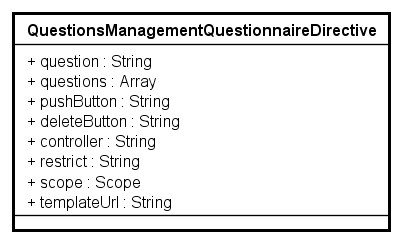
\includegraphics[scale=0.45]{UML/Classi/Front-End/QuizziPedia_Front-end_Controller_QuestionnaireQuestionsManagementController.png}
	\caption{QuizziPedia::Front-End::Controllers::QuestionnaireQuestionsManagementController}
\end{figure} \FloatBarrier
\begin{itemize}
	\item \textbf{Descrizione}: questa classe permette di gestire il recupero delle domande per il questionario;
	\item \textbf{Utilizzo}: fornisce le funzionalità per il recupero delle domande dal back-end e le rende disponibili per poter popolare le view;
	\item \textbf{Relazione con altre classi}:
	\begin{itemize}
		\item \textit{IN} \texttt{QuestionnaireQuestionsManagementDirective}: rappresenta il componente grafico che permette all'utente di:
		\begin{itemize}
			\item Effettuare delle ricerche sul database di domande;
			\item Selezionare le domande da inserire nel questionario;
			\item Mostrare le domande già inserite e permettere all'utente di eliminarle da tale lista.
		\end{itemize}
		Questo componente si presta sia per la creazione che per la modifica di un questionario;
		\item \textit{IN} \texttt{QuestionsService}: questa classe permette di ottenere domande esistenti e salvare nuove domande;
	\end{itemize}
	\item \textbf{Attributi}:
	\begin{itemize}
		\item \texttt{-} \texttt{\$scope: \$scope} \\
		Campo dati contenente un riferimento all’oggetto \$scope creato da \textit{Angular\ped{G}}, viene utilizzato come mezzo di comunicazione tra il controller e la view. Contiene gli oggetti che definiscono il model dell’applicazione;
	\end{itemize}
	\item \textbf{Metodi}:
	\begin{itemize}
		\item 
	\end{itemize}
\end{itemize}

\paragraph{QuizziPedia::Front-End::Controllers::InputToListController}
\begin{figure} [ht]
	\centering
	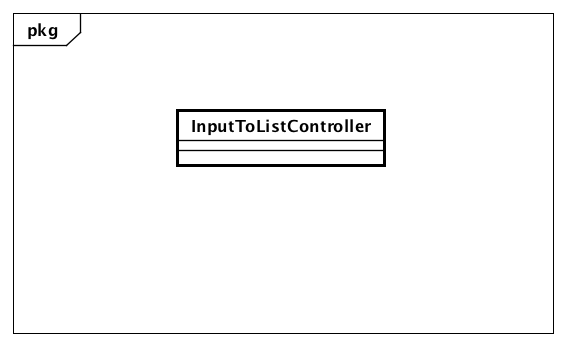
\includegraphics[scale=0.45]{UML/Classi/Front-End/QuizziPedia_Front-end_Controller_InputToListController.png}
	\caption{QuizziPedia::Front-End::Controllers::InputToListController}
\end{figure} \FloatBarrier
\begin{itemize}
	\item \textbf{Descrizione}: questa classe permette di gestire l'inserimento di una lista di risposte durante la creazione di una domanda;
	\item \textbf{Utilizzo}: fornisce le funzionalità per confermare porzioni di domanda durante la creazione;
	\item \textbf{Relazione con altre classi}:
	\begin{itemize}
		\item \textit{IN} \texttt{MultipleQuestionsView}: ;
		\item \textit{IN} \texttt{ConnectionQuestionsModelView}: ;
		\item \textit{IN} \texttt{StringsSortingQuestionsModelView}: ; 
		\item \textit{IN} \texttt{ImagesSortingQuestionsModelView}: ;
	\end{itemize}
	\item \textbf{Attributi}:
	\begin{itemize}
		\item \texttt{-} \texttt{\$scope: \$scope} \\
		Campo dati contenente un riferimento all’oggetto \$scope creato da \textit{Angular\ped{G}}, viene utilizzato come mezzo di comunicazione tra il controller e la view. Contiene gli oggetti che definiscono il model dell’applicazione;
	\end{itemize}
	\item \textbf{Metodi}:
	\begin{itemize}
		\item \texttt{+} \texttt{InputToListController(\$scope: \$scope)}: \\Metodo costruttore della classe.
		\textbf{Parametri}:
		\begin{itemize}
			\item 
		\end{itemize}
		\item \texttt{-} \texttt{putDownAnswer(): void}: \\Metodo che reagisce all'evento di aggiunta nuova risposta e la va a salvare localmente (dobbiamo decidere dove) in modo che venga caricata e visualizzata nella pagina.
	\end{itemize}
\end{itemize}

\paragraph{QuizziPedia::Front-End::Controllers::QuizEventController}
\begin{figure} [ht]
	\centering
	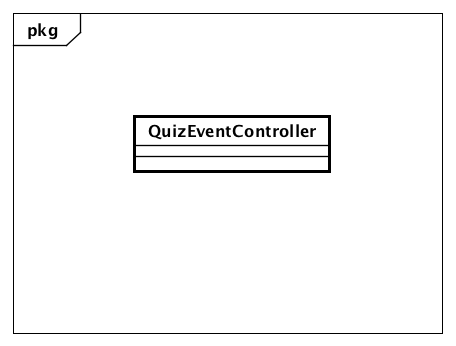
\includegraphics[scale=0.45]{UML/Classi/Front-End/QuizziPedia_Front-end_Controller_QuizEventController.png}
	\caption{QuizziPedia::Front-End::Controllers::QuizEventController}
\end{figure} \FloatBarrier
\begin{itemize}
	\item \textbf{Descrizione}: questa classe permette di reagire ai comandi dell'utente durante la gestione dei suoi questionari;
	\item \textbf{Utilizzo}: fornisce le funzionalità per reagire ai comandi dell'utente, effettua redirect alle pagine richieste, come la visualizzazione delle statistiche di un questionario e iniziare un questionario in modalità esame.
	\item \textbf{Relazione con altre classi}:
	\begin{itemize}
		\item \textit{IN} \texttt{CreationAndModifyDirective}:  
		\item \textit{OUT} \texttt{ExamModalityDirective}:
	\end{itemize}
	\item \textbf{Attributi}:
	\begin{itemize}
		\item \texttt{-} \texttt{\$scope: \$scope} \\
		Campo dati contenente un riferimento all’oggetto \$scope creato da \textit{Angular\ped{G}}, viene utilizzato come mezzo di comunicazione tra il controller e la view. Contiene gli oggetti che definiscono il model dell’applicazione;
	\end{itemize}
	\item \textbf{Metodi}:
	\begin{itemize}
		\item 
	\end{itemize}
\end{itemize}